SolVi is another very common benchmark carried out in the computational 
geodynamics literature.

This inclusion benchmark again solves a problem with a discontinuous viscosity, 
but this time the viscosity is chosen in such a way that the discontinuity is circle. 
Given the regular nature of the used by a majority of codes, 
this ensures that the discontinuity in the viscosity never aligns to cell boundaries.
This in turns leads to almost discontinuous pressures along the interface which are difficult 
to represent accurately.

Schmid \& Podlachikov (2003) \cite{scpo03}. 
derived a simple analytic solution for the pressure and velocity fields for a circular 
inclusion under simple shear 

A characteristic of the analytical solution is that the pressure is zero 
inside the inclusion, while outside it follows the relation
\[
p_m = 4 \dot{\epsilon}
\frac{\eta_m(\eta_i-\eta_m)}{\eta_i+\eta_m}
\frac{r_i^2}{r^2} \cos(2\theta)
\]
where $\eta_i$ is the viscosity of the inclusion (often taken to be 1000)
and $\eta_m1$ is the viscosity of the background media (often taken to be 1). 

One important observation with this benchmark is the fact that the velocity is not zero even far 
away from the inclusion, so that the analytical solution must be imposed on the sides.
Also, because of symmetry, it is often run on the top quadrant $x>0$, $y>0$ with 
free slip imposed on the left and bottom boundaries. 

\begin{center}
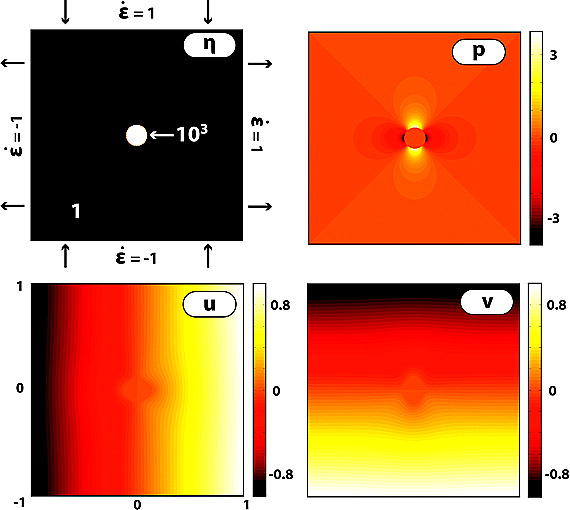
\includegraphics[width=9cm]{images/benchmark_solvi/dumg11}
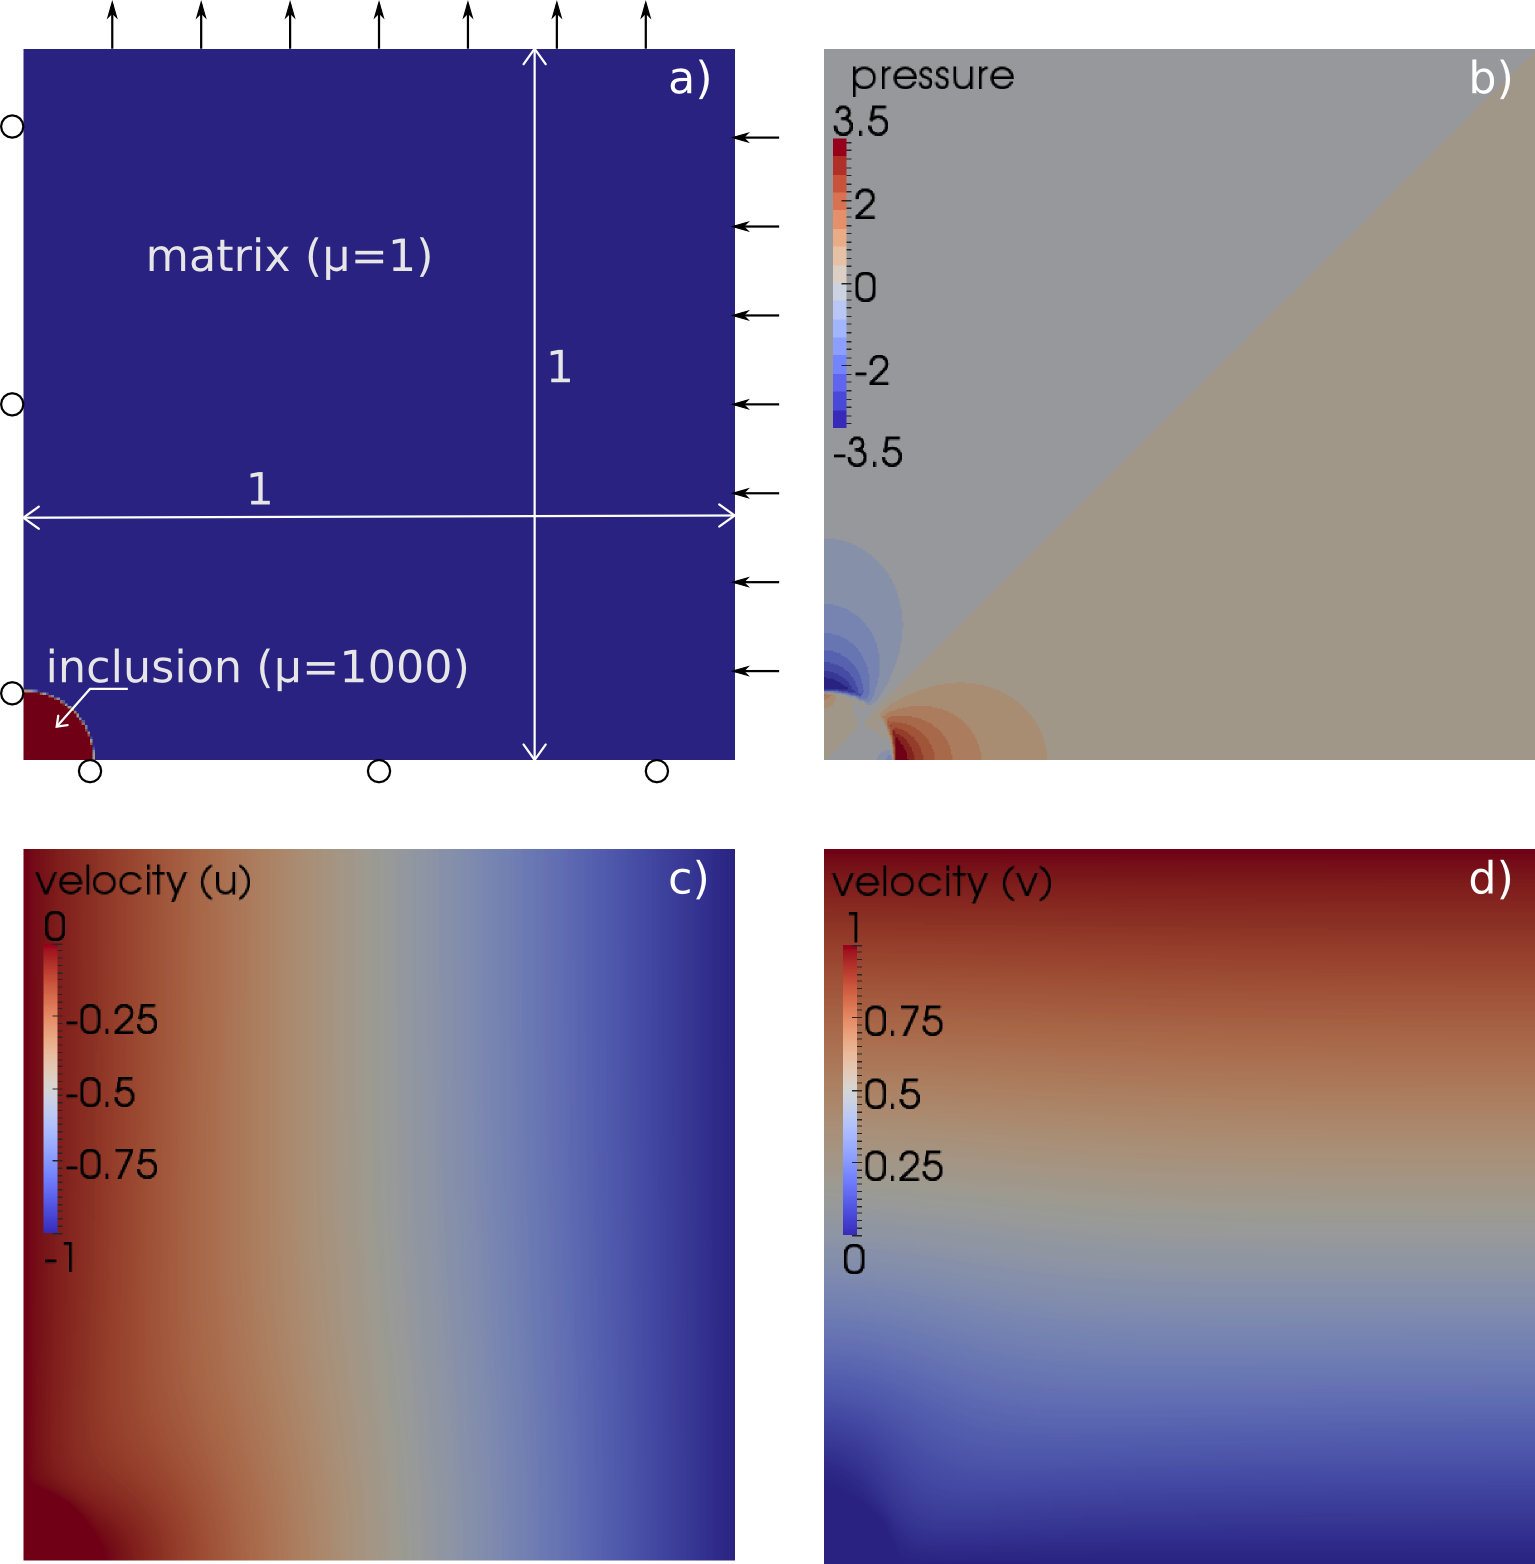
\includegraphics[width=7cm]{images/benchmark_solvi/drawing}\\
{\captionfont Left: taken from Duretz \etal (2011) \cite{dumg11}. }
\end{center}

 
\cite{kapo06,maie12,deka08,bepo10,sunh10,vosc15,demh19,aspectmanual,litu02} \stone 07
\cite{krhb12} and \cite{gemd13}.
